\section{Ergebnisse}
In diesem Kapitel sind Versuchsergebnisse dargestellt, die an dem geregelten Pendel gewonnen wurden. Dafür wurde das stabilisierte Pendel mit einem kurzen Störimpuls beaufschlagt und die Reaktion aufgezeichnet. Dieser Störimpuls erfolgte per Hand und wurde in unterschiedlichen Stärken durchgeführt, um so die einzelnen Controller testen zu können. 
\subsection{Swing-Up}
Zunächst soll anhand von Abbildung \ref{fig.Swing-Up-Plot} der Aufschwing-Vorgang betrachtet werden. Wie bereits in Kapitel \ref{Pendelidentifikation} erwähnt, vollzieht der Controller in den ersten 5 Sekunden die Identifikation des Pendels. Der dafür verwendete Impuls lässt sich bei $\theta_1$ nahe $t=0s$ erkennen. Nach diesen 5 Sekunden beginnt der Controller zunächst durch Verwendung des Zweipunktreglers und des Swing-Ups den Pendelarm in den Bereich $\left| \theta_2 \right| < 20^\circ$ zu bewegen, in welchem dann der Catcher aktiv wird, um ein Überschwingen zu verhindern. Nach einer kurzer Zeit, in der gilt $\left| \theta_2 \right| < 5^\circ$, übernimmt dann der Stabilizer mehr und mehr die Kontrolle (vgl. Kapitel \ref{Softswitch}), welcher schließlich auch $\theta_1$ auf seinen Anfangswinkel regelt.

\begin{figure}[htbp]
	\centering
	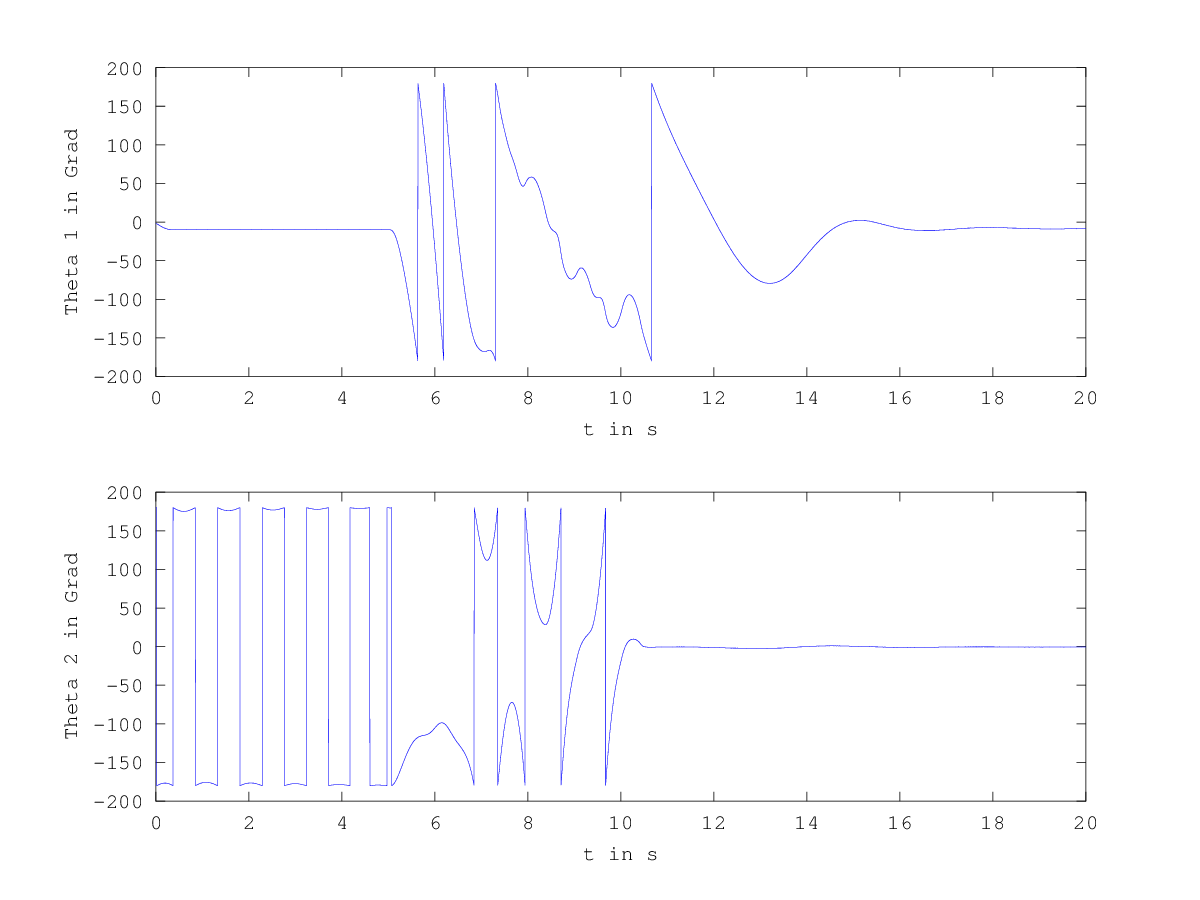
\includegraphics[width=1.\textwidth]{Grafiken/Swingup_kurz.png}
	\caption{Der Swing-Up-Vorgang}
	\label{fig.Swing-Up-Plot}
\end{figure}


\subsection{Stabilisierer}

Der Stabilisierer wird in Abb. \ref{fig.Stabilisierer-Plot} durch eine schwachen Impuls getestet, wodurch $\theta_2$ um 2 Grad ausgelenkt wurde. Dadurch bleibt der Stabilizer weiterhin aktiv und regelt die Motorspannung so, dass über das Überschwingen von $ \theta_1$ das Pendel wieder in die obere Position gebracht wird. Zudem ist zu erkennen, dass der Regler auch hier $ \theta_1$ in die Ausgangsposition zurückführt.

\begin{figure}[htbp]
	\centering
	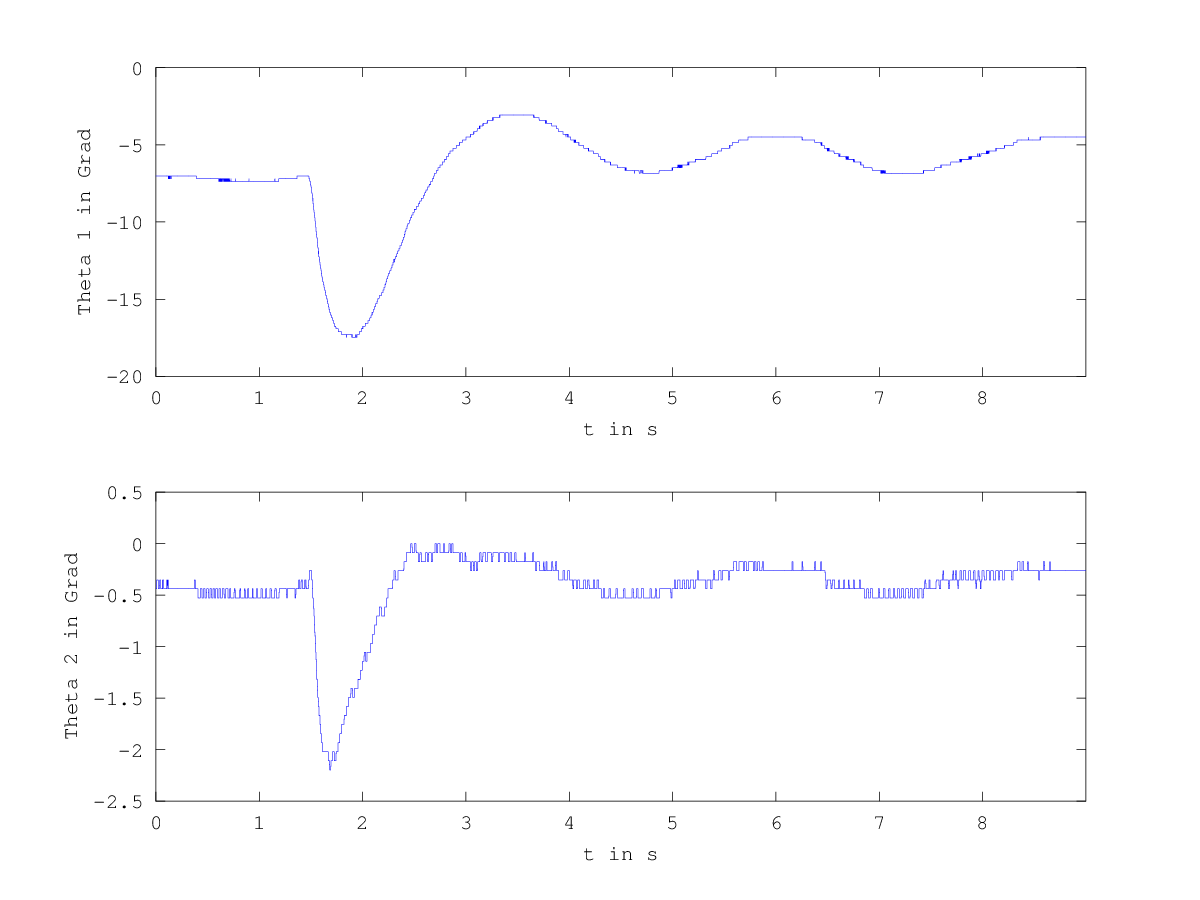
\includegraphics[width=1.\textwidth]{Grafiken/Stab_lang.png}
	\caption{Störung \textless $5^{\circ}$}
	\label{fig.Stabilisierer-Plot}
\end{figure}


\subsection{Catcher}
In Abb. \ref{fig.Catcher-Plot} sind die Auswirkungen des Reglers nach einer Störung von 9 Grad zu erkennen. Der Catcher sorgt dabei zunächst für ein schnelles Rückstellen des Pendels auf das Top Equilibrium, während nach der 3. Sekunde der Einfluss des Stabilizers steigt und dieser im Mittel $\theta_1$ gegen 0 Grad regelt, allerdings mit starken Schwingungen, um die Abweichung von $\theta_2$ auszugleichen. 
\begin{figure}[htbp]
	\centering
	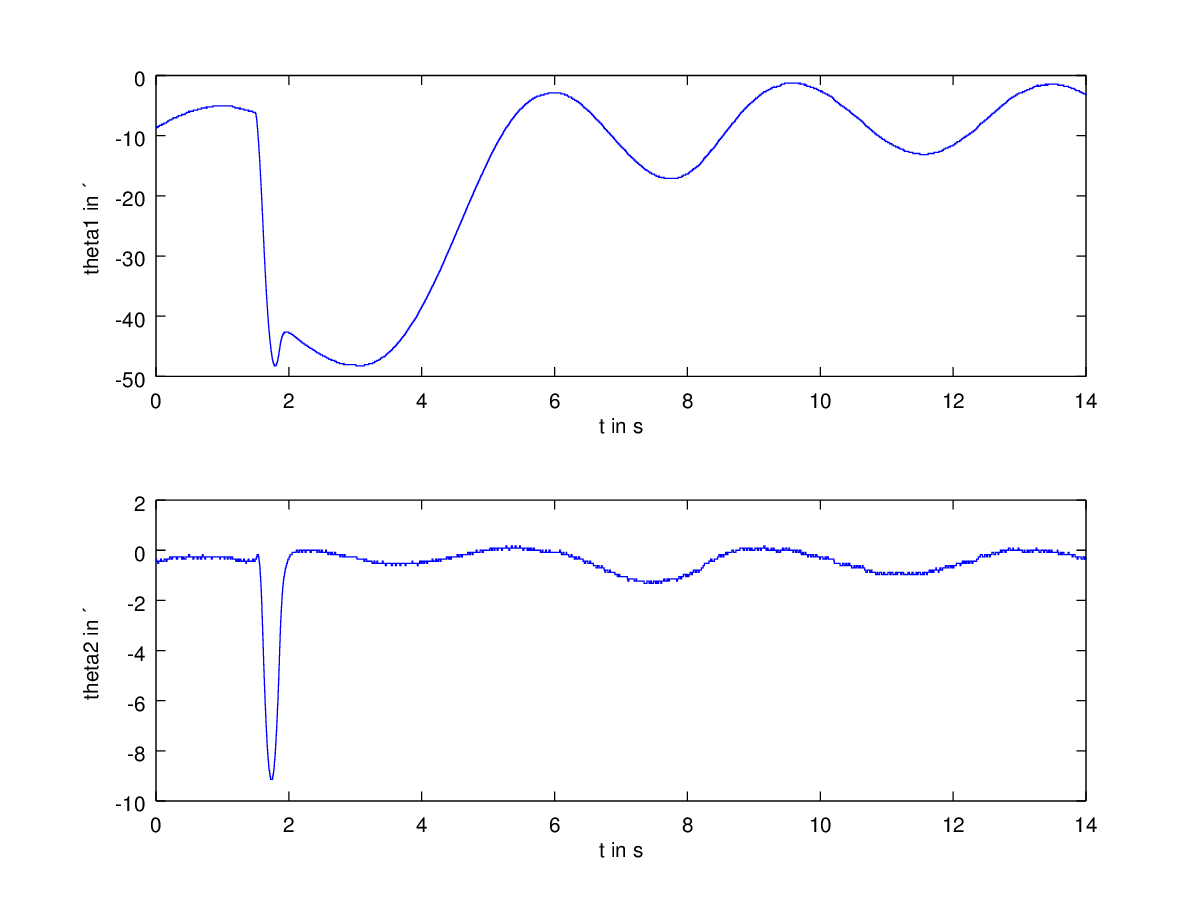
\includegraphics[width=1.\textwidth]{Grafiken/Catch_kurz.png}
	\caption{Störung \textgreater $5^{\circ}$}
	\label{fig.Catcher-Plot}
\end{figure}

\subsection{Watchdog}
Hin und wieder kommte es vor, dass das System in einen Zustand gerät, in dem es das Pendel nicht mehr fangen und in das Top Equilibrium zurückbringen kann. Dieser Zustand in in Abbildung \ref{fig.Watchdog-Plot} zu sehen. Um ein solches Verhalten zu verhindern, könnte man einen Watchdog implementieren, der anhand der Winkelgeschwindigkeit $\dot{\theta}_1$ erkennt, wenn das Pendel nicht mehr erfolgreich geregelt werden kann. Liegt der Wert von $\dot{\theta}_1$ für eine bestimmte Zeit nicht in dem Intervall $[-\epsilon,+\epsilon]$, so kann der Watchdog einen kurzzeitigen Stopp des Pendels veranlassen und es anschließend neu starten.

\begin{figure}[htbp]
	\centering
	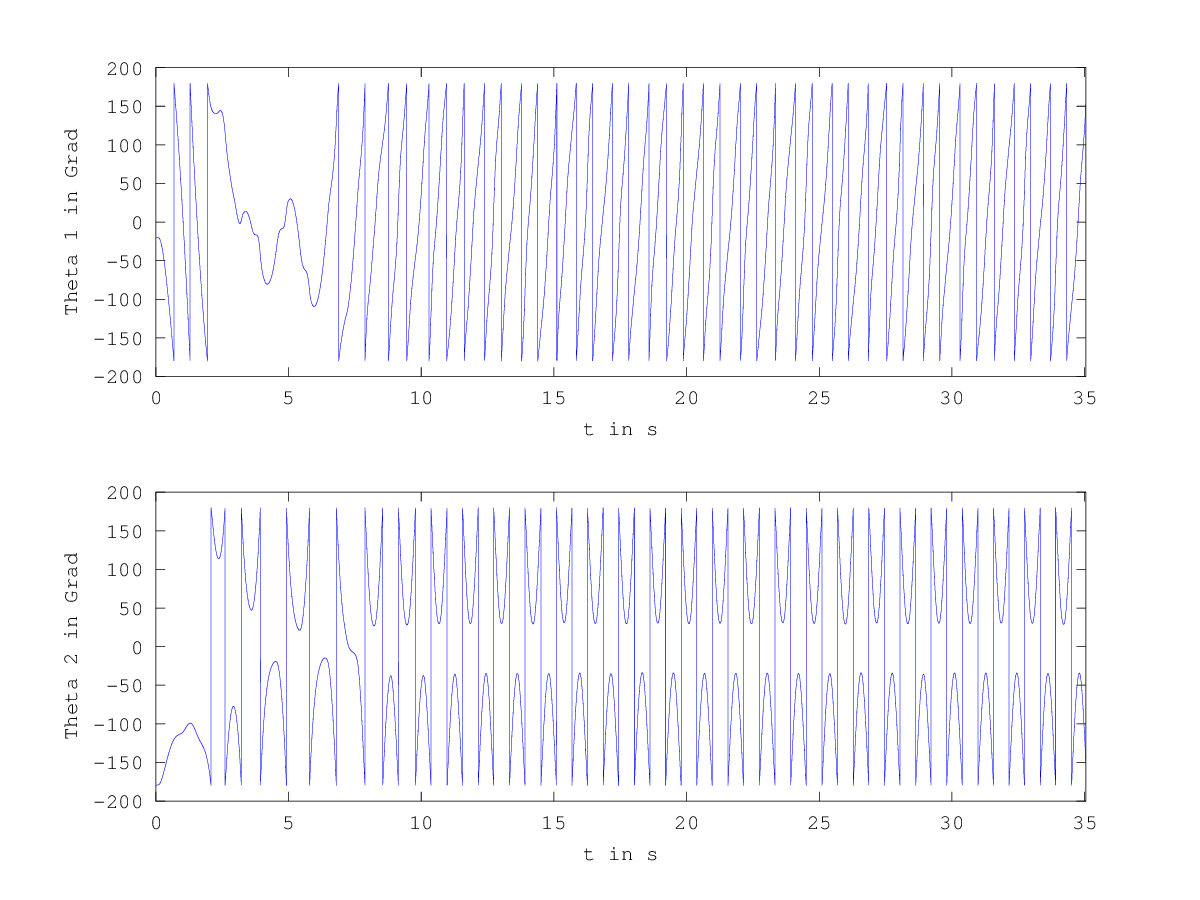
\includegraphics[width=1.\textwidth]{Grafiken/Watchdog_lang.png}
	\caption{Watchdog}
	\label{fig.Watchdog-Plot}
\end{figure}


